\section{Software Installation \& Ecosystem}
\subsection{Important Websites}
%%%%%%%%%%%%%%%%%%%%%%%%%%%%%%%%%%%%%%%%%%%%%%%%%
\frame
{
  \Large
  \begin{block}{}
    \center{\bf Important Websites}
    \begin{itemize}
      \item \href{http://libmesh.sourceforge.net}{Primary website}
      \item \href{http://github.com/libMesh/libmesh}{Revision Control \& Collaboration with GitHub}
      \item Continuous Integration with MooseBuild (from INL)
        %% \begin{itemize}
        %%   \item \href{http://buildbot.ices.utexas.edu:8010/builders/libmesh\%2Fmaster}{Vanilla Master}
        %%   \item \href{http://buildbot.ices.utexas.edu:8010/builders/libmesh\%2Fmaster%2Bsl6options}{Options}
        %% \end{itemize}
    \end{itemize}
  \end{block}
}


\frame
{
\frametitle{\url{http://libmesh.github.io}}

\centerline{
\includegraphics[width=0.85\textwidth]{webpage}}
}


\frame
{
\frametitle{\url{http://github.com/libMesh/libmesh}}

\centerline{\includegraphics[width=0.85\textwidth]{trivia/github_site}}
}


\frame
{
\frametitle{MooseBuild Testing Integrated with GitHub}

\centerline{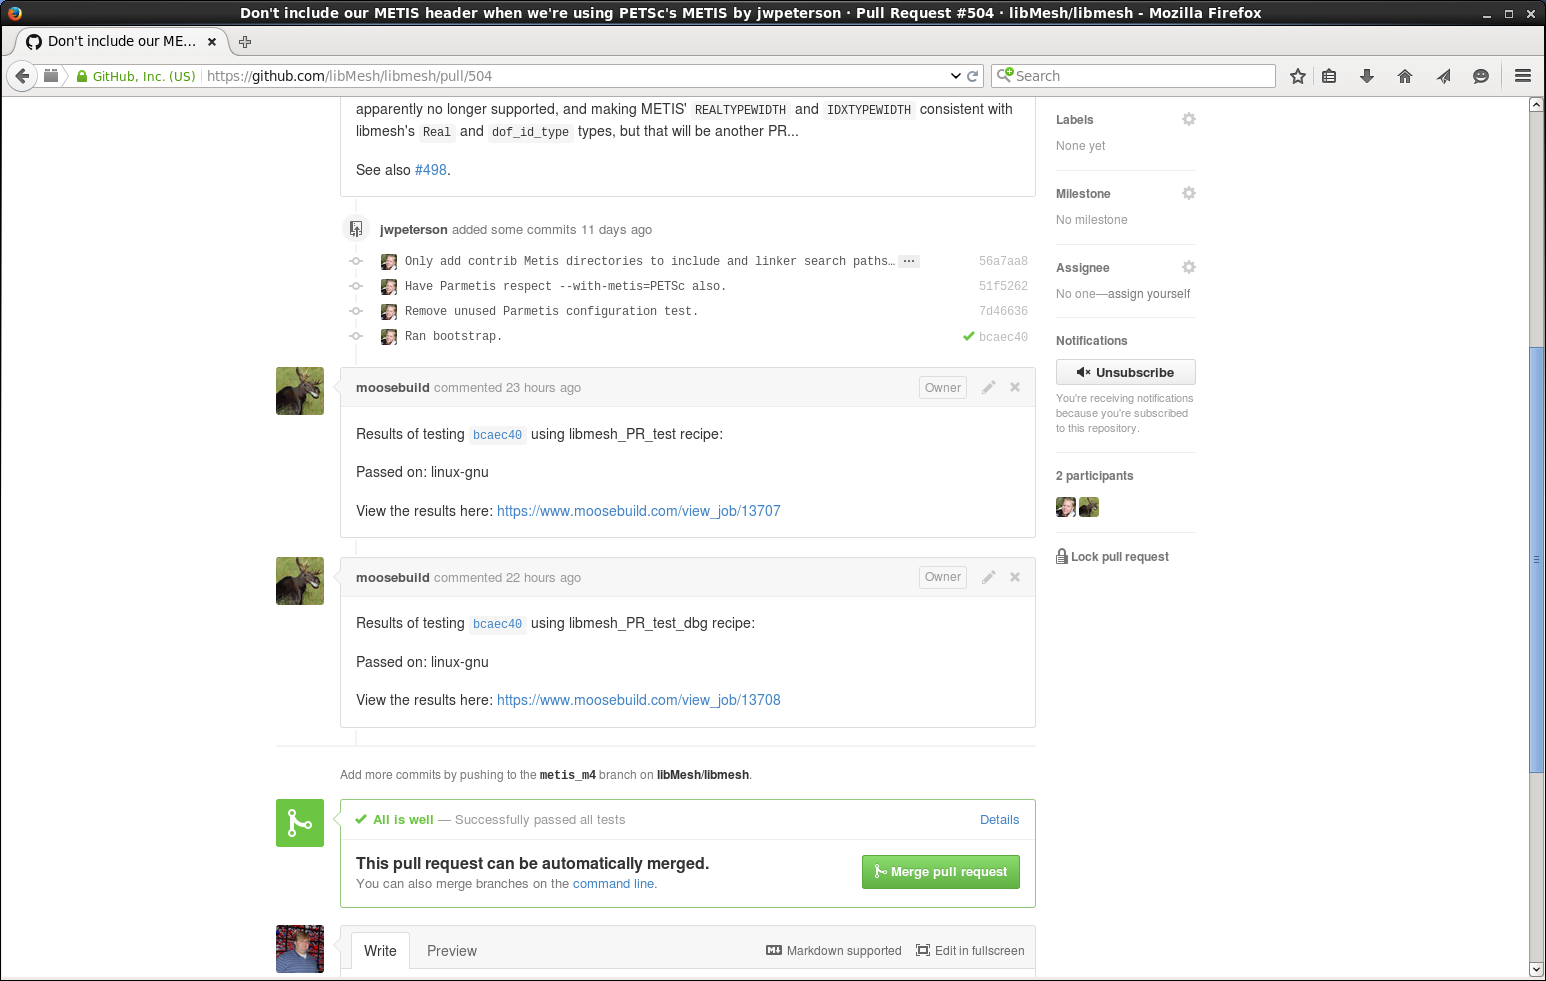
\includegraphics[width=0.85\textwidth]{moose_build}}
}



\subsection{Compiling the library}
\frame
{
  \Large
  \begin{block}{}
    \center{\bf Building \libMesh{}}
  \end{block}
}


\begin{frame}[fragile]
  \frametitle{Getting the \libMesh{} Source}

  \begin{block}{}
    \begin{itemize}
    \item \textbf{Blessed, Stable releases:}

      Download prepackaged releases from

      \scriptsize{\url{http://github.com/libMesh/libmesh/releases}}
      \normalsize
    \item \textbf{Development tree:}

      Grab the latest source tree from GitHub:
      \begin{lstlisting}[language=bash]
$ git clone git://github.com/libMesh/libmesh.git
      \end{lstlisting}
    \end{itemize}
  \end{block}
\end{frame}

\begin{frame}
  \frametitle{\libMesh{} Suggested Dependencies}
  \begin{itemize}
    \item  \texttt{MPI} is of course required for shared-memory parallelism.
    \item Out of the box, \libMesh{} will build with support for serial linear systems.
    \item Highly recommended you first install \texttt{PETSc} and/or \texttt{Trilinos}, which \libMesh{} uses for solving linear systems in parallel.
      \item Other recommended, optional packages are:
        \begin{itemize}
          \item \texttt{SLEPc}: eigenvalue support on top of \texttt{PETSc}.
          \item Intel's Threading Building Blocks for shared-memory multithreading.
        \end{itemize}
  \end{itemize}
\end{frame}

\begin{frame}[fragile]
  \frametitle{Building \libMesh{} from source}

  \begin{block}{Unpack, Configure, Build, Install, \& Test}
    \begin{lstlisting}[language=bash]
# unpack the distribution
$ tar jxf libmesh-0.9.1.tar.bz2 && cd libmesh-0.9.1
# configure, install into the current directory
$ ./configure --prefix=$PWD/install
# build & install
$ make -j 4 && make -j 4 install
# run all the examples, but only the optimized flavor
$ make -j 4 check METHODS=opt
    \end{lstlisting}
  \end{block}
\end{frame}



\begin{frame}[fragile]
  \frametitle{Building \libMesh{} from source}

  \begin{block}{Advanced Configurations}
    \begin{lstlisting}[language=bash]
# unpack the distribution
$ tar jxf libmesh-0.9.1.tar.bz2 && cd libmesh-0.9.1
# build in a subdirectory, allows multiple simultaneous builds
$ mkdir -p clang && cd clang
# configure specifing optional packages & compilers
$ ../configure --prefix=$PWD/install \
               --with-glpk-include=/opt/local/include \
               --with-glpk-lib=/opt/local/lib \
               --with-vtk-include=/opt/local/include/vtk-5.10 \
               --with-vtk-lib=/opt/local/lib/vtk-5.10 \
               --with-eigen-include=/opt/local/include/eigen3 \
               --with-cxx=clang++-mp-3.3 --with-cc=clang-mp-3.3 \
               --disable-fortran
# build & install
$ make -j 4 && make -j 4 install
    \end{lstlisting}
  \end{block}
\end{frame}



\begin{frame}[fragile,shrink]
  \frametitle{Building \libMesh{} from source}

  \begin{block}{Testing the Installation}
    \begin{lstlisting}[language=bash]
$ make -j 4 installcheck
Making installcheck in include
Making installcheck in libmesh

Checking for standalone headers in installed tree ...

Testing Header libmesh/libmesh_config.h ...            [   OK   ]
Testing Header base/auto_ptr.h ...                     [   OK   ]
Testing Header base/dirichlet_boundaries.h ...         [   OK   ]
Testing Header base/dof_map.h ...                      [   OK   ]
Testing Header base/dof_object.h ...                   [   OK   ]
...

Checking for self-sufficient examples...

Testing examples in /tmp/libmesh-0.9.1/_inst/examples
Testing example installation adaptivity/ex1 ...        [   OK   ]
Testing example installation adaptivity/ex2 ...        [   OK   ]
Testing example installation adaptivity/ex3 ...        [   OK   ]
Testing example installation adaptivity/ex4 ...        [   OK   ]
Testing example installation adaptivity/ex5 ...        [   OK   ]
...
    \end{lstlisting}
  \end{block}
\end{frame}



\subsection{Compiling Applications}
\frame
{
  \Large
  \begin{block}{}
    \center{\bf Getting Started with \libMesh{} Applications}
  \end{block}
}



\begin{frame}[fragile,shrink]
  \frametitle{The \libMesh{} installation}

  \begin{block}{Installation Tree}
    \begin{lstlisting}[language=bash]
# henceforth we assume LIBMESH_DIR points to the installation path
$ cd $LIBMESH_DIR
$ ls
Make.common contrib     examples    lib
bin         etc         include     share
$ ls lib | grep mesh
libmesh_dbg.0.dylib
libmesh_dbg.dylib
libmesh_dbg.la
libmesh_devel.0.dylib
libmesh_devel.dylib
libmesh_devel.la
libmesh_opt.0.dylib
libmesh_opt.dylib
libmesh_opt.la
$ ls lib/pkgconfig
Make.common      libmesh-devel.pc libmesh-opt.pc   libmesh.pc
libmesh-dbg.pc   libmesh-oprof.pc libmesh-prof.pc  netcdf.pc
    \end{lstlisting}
  \end{block}
\end{frame}



\begin{frame}[fragile,shrink]
  \frametitle{The \libMesh{} installation}

  \begin{block}{Compiling Simple Applications with \texttt{pkg-config}}
    \begin{lstlisting}[language=bash]
# make sure pkg-config can find the libMesh configuration
$ export PKG_CONFIG_PATH=$LIBMESH_DIR/lib/pkgconfig:$PKG_CONFIG_PATH

# copy the first example program
$ cp -r $LIBMESH_DIR/examples/introduction/ex1 . && cd ex1

# see what we've got
$ ls
Makefile introduction_ex1.C run.sh

# compile against the full debug version of libMesh
$ mpicxx -o introduction_ex1 introduction_ex1.C \
  `pkg-config --cflags --libs libmesh-dbg`

# compile against the default, optimized version of libMesh
$ mpicxx -o introduction_ex1 introduction_ex1.C \
  `pkg-config --cflags --libs libmesh`
    \end{lstlisting}
  \end{block}
\end{frame}






\begin{frame}[fragile,shrink]
  \frametitle{The \libMesh{} installation}

  \begin{block}{Compiling Simple Applications with \texttt{libmesh-config}}
    \begin{lstlisting}[language=bash]
# we support a similar utility, libmesh-config, which predates
# pkg-config support. this is similar, but also can report the
# compiler used.
$ PATH=$LIBMESH_DIR/bin:$PATH

$ libmesh-config
usage: libmesh-config --cppflags --cxxflags --include --libs
       libmesh-config --cxx
       libmesh-config --cc
       libmesh-config --fc
       libmesh-config --fflags
       libmesh-config --version
       libmesh-config --host

# get the name of the compiler used, as passed to ./configure
$ libmesh-config --cxx
mpicxx
    \end{lstlisting}
  \end{block}
\end{frame}



\begin{frame}[fragile,shrink]
  \frametitle{The \libMesh{} installation}

  \begin{block}{Compiling Applications with \texttt{make}}
    \begin{lstlisting}[language=bash]
# copy the first example program
$ cp -r $LIBMESH_DIR/examples/introduction/ex1 . && cd ex1

# compile against the default, optimized version of libMesh
$ make
Compiling C++ (in optimized mode) introduction_ex1.C...
Linking example-opt...

# compile against the full debug version of libMesh
$ make METHOD=dbg
Compiling C++ (in debug mode) introduction_ex1.C...
Linking example-dbg...
    \end{lstlisting}
  \end{block}
\end{frame}



\begin{frame}[fragile,shrink]
  \frametitle{A first \libMesh{} application}
  \begin{lstlisting}
#include <iostream>
#include "libmesh/libmesh.h"
#include "libmesh/mesh.h"

using namespace libMesh;

int main (int argc, char** argv)
{
  LibMeshInit init (argc, argv);

  if (argc < 4)
    {
      if (libMesh::processor_id() == 0)
        std::cerr << "Usage: " << argv[0] << " -d 2 in.mesh [-o out.mesh]"
                  << std::endl;

      libmesh_error();
    }

  Mesh mesh(init.comm());

  mesh.read (argv[3]);

  mesh.print_info();

  if (argc >= 6 && std::string("-o") == argv[4])
    mesh.write (argv[5]);

  return 0;
}
  \end{lstlisting}
\end{frame}



\begin{frame}[fragile,shrink]
  \frametitle{A first \libMesh{} application}
  \begin{lstlisting}[language=bash]
# copy & build the example
$ cp -r $LIBMESH_TUTORIAL/basic .
$ cd basic
$ make
Compiling C++ (in optimized mode) introduction_ex1.C...
Linking example-opt...

# run the example, reading a trivial mesh and writing output
$ ./example-opt -d 3 \
  $LIBMESH_DIR/share/reference_elements/3D/one_hex27.xda -o out.exo
 Mesh Information:
  mesh_dimension()=3
  spatial_dimension()=3
  n_nodes()=27
    n_local_nodes()=27
  n_elem()=1
    n_local_elem()=1
    n_active_elem()=1
  n_subdomains()=1
  n_partitions()=1
  n_processors()=1
  n_threads()=1
  processor_id()=0
  \end{lstlisting}
\end{frame}
